\chapter{Программирование Тестера}
\label{sec:config}
\section{Конфигурирование Тестера}
Пакет программного обеспечения для Тестера доступен с исходными кодами. Компиляцией модулей управляют с помощью 
Makefile. Разработка была сделана в операционной системе Linux Ubuntu с GNU toolchain (gcc версия 4.5.3). Можно 
использовать и другие операционные системы, например, Windows. Чтобы загрузить скомпилированные данные во Flash 
память и память EEprom программой \lcmd{avrdude} (версия 5.11svn) загружают Makefile и указывают \lcmd{make upload}. Программа 
\lcmd{avrdude} \cite{avrdude} доступна для операционных систем Linux и Windows. C-компилятор GNU gcc также поддерживается 
программным обеспечением AVR Studio и WinAVR \cite{winavr1},\cite{winavr2} в операционной системе Windows. Вы можете 
запрограммировать ATmega данными (.hex и.eep) также и другими инструментами, но только моя версия Makefile 
автоматически загрузит правильные данные в выбранный микроконтроллер. Avrdude загружает данные в ATmega, если 
Signature Bytes, подключённого ATmega, идентичны выбранному. Если Вы измените Makefile, то все программное 
обеспечение нужно будет скомпилировать вновь, указав команду \lcmd{make} или \lcmd{make upload}. Программное обеспечение, 
скомпилированное для ATmega8, не работает на ATmega168. Программное обеспечение, скомпилированное для ATmega328, 
не работает на ATmega168! Исключением из этого правила является программное обеспечение, скомпилированное для 
ATmega168, эти данные могут также использоваться для ATmega328 без изменений. Будьте внимательны, если Вы не 
используете мой Makefile. 

При правильном выборе установок, мое программное обеспечение запускается на недоработанных аппаратных средствах 
от Markus F.
Вы должны установить PARTNO=M8, и \textbf{ НЕ} устанавливать опции NO\_AREF\_CAP и PULLUP\_DISABLE. 
Тактовая частота может также быть установлена \(8~MHz\) с фьюзами, указывающими, что кварц не требуется! 

Для конфигурирования программного обеспечение Вашего Тестера доступны следующие опции, определенные в Makefile.


\begin{description} \setlength{\itemsep}{0em}
  \item[PARTNO] Описывает целевой микроконтроллер:\\
         m8 = ATmega8\\
         m168 or m168p	= ATmega168\\
         m328 or m328p	= ATmega328\\
         m644 or m644p	= ATmega644\\
         m1284p		= ATmega1284\\
         m1280		= Atmega1280\\
         m2560		= ATmega2560\\   
Пример:  PARTNO = m168

  \item[WITH\_MENU] Активируется меню выбора функций для ATmega328. Вы сможете выбрать некоторые дополнительные 
  функции работы прибора из меню при длительном (\textgreater~\(0,5~s\)) нажатии кнопки \textbf{ TEST}.\\
Пример: CFLAGS += -DWITH\_MENU

 \item[MAX\_MENU\_LINES]
Эта опция указывает максимальное количество строк для выбора отображаемых функций меню.
Обычно количество строк выводится в соответствии с количеством строк дисплея.
Поскольку пунктов меню больше чем строк доступных на дисплее, выбор циклически прокручивается.
Обработка вывода на дисплей во время циклического обмена требует значительного времени,
особенно для больших цветных многострочных дисплеев.
Ограничивая количество строк этой опцией, время вывода во время выбора меню может быть уменьшено,
что ускоряет работу.
Значение для этой опции по умолчанию равно 5.\\
Пример: CFLAGS += -DMAX\_MENU\_LINES=3

  \item[WITH\_ROTARY\_SWITCH] Использование поворотного инкрементального энкодера в
качестве опции для быстрого доступа в меню дополнительных функций (смотрите описание
~\ref{fig:RotExt} в разделе Улучшения и расширения к прибору).
Если количество циклов переключения контактов, за каждый оборот Вашего энкодера, соответствует количеству 
фиксированных позиций, Вы должны установить значение WITH\_ROTARY\_SWITCH=2 или 3. Если полный цикл переключения 
требует поворота энкодера на две фиксированные позиции, то опцию WITH\_ROTARY\_SWITCH нужно установить =1.
Установка опции WITH\_ROTARY\_SWITCH равной 5 выбирает максимальное разрешения энкодера. Каждый цикл переключения 
в двух каналах дает 4 результата состояния счетчиков. Обычно этот параметр полезен только для энкодеров без фиксации.
Значение опции WITH\_ROTARY\_SWITCH равной 4 необходимо, если установлено две отдельные кнопки 
\inquotes{Вверх} и \inquotes{Вниз} вместо энкодера. Не используйте значение 4 если у Вас установлен энкодер!\\
Пример: CFLAGS += -DWITH\_ROTARY\_SWITCH=1

  \item[CHANGE\_ROTARY\_DIRECTION] Опция позволяет программно изменить направление движения курсора при повороте 
энкодера. Опция CHANGE\_ROTARY\_DIRECTION равнозначна физической перестановке выводов каналов энкодера.\\
Пример: CFLAGS += -DCHANGE\_ROTARY\_DIRECTION

  \item[ROTARY\_2\_PIN=PD2] Опция позволяет программно изменить назначение порта PD1. Лучшее решение для подключения 
инкрементального энкодера это порт PD1 и PD3. Tак как первый проект использовал PD2 вместо PD1, то 
вернуться к старому варианту Вы можете, переопределив PD1 и установив следующую опцию настройки по умолчанию: 
CFLAGS += -DROTARY\_2\_PIN=PD2. Для второго канала энкодера можно использовать любой 
свободный порт PD указав его номер.\\
Пример: CFLAGS += - DROTARY\_2\_PIN=PD2
 
  \item[UI\_LANGUAGE] Определяет выбранный язык\\
В настоящее время доступны:\\
    LANG\_BRASIL, LANG\_CZECH, LANG\_DANISH, LANG\_DUTCH, LANG\_ENGLISH, \\
    LANG\_GERMAN, LANG\_HUNGARIAN, LANG\_ITALIAN, LANG\_LITHUANIAN, \\
    LANG\_POLISH, LANG\_RUSSIAN, LANG\_SLOVAK, LANG\_SLOVENE, \\
    LANG\_SPANISH и LANG\_UKRAINIAN. Русский или украинский язык требует LCD-дисплей с 
кириллической кодировкой.\\
Пример:  UI\_LANGUAGE = LANG\_RUSSIAN

  \item[LCD\_CYRILLIC] Необходима для некоторых LCD-дисплеев с кодировкой для европейских или кириллических языков.
Символы \(\mu\) и \(\Omega\) отсутствуют в их кодировке. Если Вы выбрали эту опцию, то оба символа 
отображаются на LCD-дисплее программно.\\
Пример: CFLAGS += -DLCD\_CYRILLIC

  \item[LCD\_DOGM] Должна быть установлена, если применяется LCD-дисплей с контроллером ST7036 (тип DOG-M). 
Контрастность LCD-дисплея устанавливают командами программного обеспечения. 
Если значение контраста изменено не корректно и на дисплее ничего не видно, то Вы можете попытаться 
его отрегулировать при просмотре дисплея под большим углом. Если и это не решило проблему, то надо переписать
содержимое EEPROM при помощи ISP программатора.\\
Пример: CFLAGS += -DLCD\_DOGM

  \item[FOUR\_LINE\_LCD] Предусматривает установку символьного 4x20 LCD для более детального отображения 
дополнительной информации. Для графических контроллеров 128х64 установка этой опции не обязательна, так как
для них информация выводится всегда в четыре строки.\\
Пример: CFLAGS += -DFOUR\_LINE\_LCD

  \item[DD\_RAM\_OFFSET] Некоторые символьные дисплеи используют различные DD-RAM стартовые адреса для начала каждой строки.
Обычно для строки 1 начальный адрес DD-RAM 0.
Некоторые дисплеи, например TC1604 или TC1602 используют 128 (0x80) для начала строки 1.
Эта опция может разрешить такую проблему. \\
Пример: CFLAGS += -DDD\_RAM\_OFFSET = 128

  \item[LCD\_LINE\_LENGTH=20] Задает количество символов, выводимых в одну строку для отображения на LCD.
Следует заметить, что для графических индикаторов 128х64 выводится 16 символов в строку. 
Этот параметр игнорируется для таких индикаторов. \\
Пример: CFLAGS += -DLCD\_LINE\_LENGTH=20

  \item[DPAGE\_MODE] При применении индикатора 4x20 LCD или графического индикатора 128х64 точек, позволяет 
изменить способ выбора пунктов меню: неподвижный курсор в третьей строке с перемещением пунктов меню или 
перемещаемый курсор по пунктах меню. \\
Пример: CFLAGS += -DPAGE\_MODE
 
  \item[WITH\_LCD\_ST7565] Эта опция должна устанавливаться при использовании графического 128x64 точек LCD с 
контроллером ST7565, который подключен по последовательному интерфейсу SPI или I\textsuperscript{2}C. Для этого типа дисплея должны быть 
установлены дополнительные параметры, которые указаны в таблице~\ref{tab:cod-display}.
При использовании контроллера ST7565 Вы должны установить значение этого параметра 1 или 7565. 
Вы также можете использовать совместимый контроллер SSD1306 вместо контроллера ST7565.
Это должно быть сделано путем установки переменной WITH\_LCD\_ST7565 = 1306.
Поддерживается дисплей с контроллером PCF8812 или PCF8814, если опция установлена правильно.
Также может быть подключен дисплей с контроллером ST7920 или NT7108.
Для контроллера NT7108 нужно использовать последовательно-параллельный преобразователь интерфейсов 
74HC(T)164 или 74HC(T)595. \\
Пример: WITH\_LCD\_ST7565 = 1

 \item[LCD\_INTERFACE\_MODE] Для контроллера SSD1306 возможно использование интерфейса I\textsuperscript{2}C с адресом 0x3c
вместо 4-проводного SPI интерфейса. Для использования такой возможности, значение параметра 
LCD\_INTERFACE\_MODE установите равным 2.
Для контроллера ST7920, при подключении по специальному последовательному интерфейсу, этот параметр должен быть установлен равным 5.
Все возможные, на текущий момент, значения LCD\_INTERFACE\_MODE и WITH\_LCD\_ST7565 указаны в таблице~\ref{tab:cod-display}.

\begin{table}[H]
  \begin{center}
    \begin{tabular}{| c | c | c | c|}
    \hline
  Тип дисплея         &  Итерфейс        & WITH\_LCD\_ST7565 & LCD\_INTERFACE\_MODE \\
    \hline
    \hline
  символьный 16x2,    & 4-Bit parallel   & Параметр        &  Параметр отключён (1) \\
  символьный 20x4     & 4-Bit SPI        & отключён (0)    &    4  \\
                     & I\textsuperscript{2}C &            &   2 \\
    \hline
  графический ST7565  & 4-Bit SPI        & 1 или 7565      &  Параметр отключён (4) \\
    \hline
  графический ST7565  & I\textsuperscript{2}C & 1 или 7565 &   2 \\
    \hline
  графический SSD1306 & 4-Bit SPI        & 1306            &  Параметр отключён (4) \\
    \hline
  графический SSD1306 & I\textsuperscript{2}C & 1306       &   2 \\
    \hline
  графический ST7920  & 4-Bit parallel   & 7920            &  Параметр отключён (1) \\
    \hline
  графический ST7920  & 2-Bit serial     & 7920            &   5 \\
    \hline
  графический NT7108  & 8-Bit parallel   & 7108            &  Параметр отключён (6) \\
      или KS0108      &    + 74HCT164    &                 &     \\
    \hline
  графический PCF8812 & SPI              &   8812          &  Параметр отключён (4) \\
    \hline
  графический PCF8814 & SPI              &   8814          &  Параметр отключён (4) \\
                    & I\textsuperscript{2}C & 8814         &   2 \\
                      & 3-проводной      &   8814          &   3 \\
    \hline
  графический ILI9163 & 4-Bit SPI        &   9163          &  Параметр отключён (4) \\
  128x128 Color     &                 &                   &              \\
    \hline
  графический ST7735 & 4-Bit SPI         &   7735          &  Параметр отключён (4) \\
  128x160 Color     &                 &                   &              \\
    \hline
    \end{tabular}
  \end{center}
  \caption{Настройка интерфейса подключаемого дисплея}
  \label{tab:cod-display}
\end{table}

В таблице значение кода в скобках указано для справки и используется внутрипрограммно.
По этому, параметр, значение которого указано в скобках, при использовании такого дисплея 
должен быть отключён в makefile.\\
Пример: CFLAGS += -DLCD\_INTERFACE\_MODE=2

 \item[LCD\_SPI\_OPEN\_COL] С опцией LCD\_SPI\_OPEN\_COL уровень сигнала данных SPI интерфейса
не достигает непосредственно уровня VCC.
Низкий уровень сигнала равен уровню GND, а высокий уровень ограничен использованием \inquotes{подтягивающих} резисторов ATmega.
Если опция PULLUP\_DISABLE установлена, то требуется внешний резистор для сигнала RESET.
Для других сигналов внутренние \inquotes{подтягивающие} резисторы ATmega используются, 
даже если опция PULLUP\_DISABLE установлена.\\
Пример: CFLAG += -DLCD\_SPI\_OPEN\_COL

  \item[LCD\_I2C\_ADDR] Адрес для контроллера SSD1306 при подключении по интерфейсу I\textsuperscript{2}C . Вы можете выбрать два 
варианта: 0x3c если вывод контроллера D/C подключен к GND и 0x3d если к VCC.\\ 
Пример: CFLAGS += -DLCD\_I2C\_ADDR=0x3d

  \item[LCD\_ST7565\_RESISTOR\_RATIO] Эта опция позволяет выбирать соотношение резисторов, для внутреннего 
регулятора напряжения контроллера ST7565.
На практике обычно эти значения от 4 до 7.
Возможна установка значений от 0 до 7.\\
Пример: LCD\_ST7565\_RESISTOR\_RATIO = 4

  \item[LCD\_ST7565\_H\_FLIP] Эта опция позволяет перевернуть выводимое на LCD изображение по горизонтали.
Возможные значения: 0 - без поворота; 1 - с переворотом.\\
Пример: CFLAGS += -DLCD\_ST7565\_H\_FLIP = 1
   
  \item[LCD\_ST7565\_H\_OFFSET] Горизонтальное адресное пространство контроллера (132) больше чем видимая область LCD (128).
В зависимости от конструктивной особенности модуля, для правильного отображения, может понадобиться задать значения 
0, 2 или 4.\\
Пример: CFLAGS += -DLCD\_ST7565\_H\_OFFSET = 4

  \item[LCD\_ST7565\_V\_FLIP] Эта опция позволяет перевернуть выводимое на LCD изображение по вертикали.
Значение 0 - без переворота, 1 - с переворотом изображения по вертикали.\\
Пример: CFLAGS += -DLCD\_ST7565\_V\_FLIP = 1

  \item[VOLUME\_VALUE] Для контроллеров ST7565 или SSD1306 можно переопределить значение контрастности.
Для контроллера ST7565 значение должно быть между 0 и 63. Для контроллера SSD1306 значение нужно
выбрать от 0 до 255.\\
Пример: CFLAGS += -DVOLUME\_VALUE = 25

  \item[LCD\_ST7565\_Y\_START] С этой опцией Вы можете установить первую строку правильно, 
т.е. вверху экрана. Первая строка в некоторых версиях дисплеев смещена к середине видимой области. 
Для такого варианта дисплея, Вы можете сместить первою строку к верху видимой области, 
если опция установлена 32 (половина высоты видимой области).\\  
Пример: CFLAGS += -DLCD\_ST7565\_Y\_START = 32

  \item[LCD\_CHANGE\_COLOR] Эта опция расширяет функции меню и позволяет 
изменить цвет фона и цвет выводимой информации. Если значение установлено равным 2, то цвета синий 
и красный меняются местами. Вы можете выбрать эту опцию только для цветных дисплеев (контроллер ST7735 или ILI9163).\\
Пример: CFLAGS += -DLCD\_CHANGE\_COLOR=1

  \item[LCD\_BG\_COLOR] Задав 16-битное значение, можно выбрать цвет фона.
Как правило, старшие 5 битов используются для красного цвета, средние 6 битов используются для зеленого цвета, 
а младшие 5 битов используются для синего цвета. Иногда биты для красного и синего цвета меняются местами.
Вы можете выбрать эту опцию только для цветных дисплеев (контроллер ST7735 или ILI9163).\\
Пример: CFLAGS += -DLCD\_BG\_COLOR=0x000f

  \item[LCD\_FG\_COLOR] Этим 16-битным значением Вы можете выбрать цвет выводимой информации.
В приведенном примере -- белый цвет для текста и символов.
Вы можете выбрать эту опцию только для цветных дисплеев (контроллер ST7735 или ILI9163).\\
Пример: CFLAGS += -DLCD\_FG\_COLOR=0xffff

  \item[FONT\_8X16] Вы должны выбрать размер шрифта для графического контроллера.
  Доступны следующие размеры символов шрифтов с именем \inquotes{FONT\_} из нижеперечисленных (ширина Х высота).
Размеры 6X8, 8X8, 7X12, 8X12, 8X14, 8X15, 8X15thin, 8X16 и 16X16thin сейчас доступны.
Шрифты 8х16 и 8х16thin наиболее эффективно используют графическое пространство дисплея 128x64 пикселя.\\
Пример: CFLAGS += -DFONT\_8X16

  \item[CFLAGS += -DBIG\_TP] Опция позволяет незначительно увеличить шрифт номеров выводов ТП на графическом 
изображении.\\
Пример: CFLAGS += -DBIG\_TP

  \item[CFLAGS += -DINVERSE\_TP] Опция позволяет вывести номера выводов на графическом изображении инверсно - \inquotes{черное} 
на белом». Использование опции INVERSE\_TP автоматически отключает опцию BIG\_TP, поскольку требуется место 
для обрамления.\\
Пример: CFLAGS += -DINVERSE\_TP
  
  \item[STRIP\_GRID\_BOARD] Эта опция позволяет изменить назначения выводов порта D для подключения дисплея.
Более подробное описание Вы можете найти в описании аппаратных средств главы~\ref{sec:hardware} на 
странице~\pageref{sec:hardware}.
Вы также можете выбрать альтернативное подключение выводов ATmega к графическому индикатору.
Для китайского клона \inquotes{T5} Вы должны установить значение STRIP\_GRID\_BOARD=5.
При альтернативном назначении контактов для графического дисплея подключение кнопки \textbf{ TEST} остается неизменным.\\
Пример: CFLAGS += -DSTRIP\_GRID\_BOARD

  \item[WITH\_SELFTEST] Если Вы выбираете эту опцию, программное обеспечение будет включать функцию самодиагностики. 
  Самодиагностика будет начата, если Вы соедините все 3 испытательных порта вместе \inquotes{перемычкой} и нажмете кнопку 
\textbf{ TEST}. Если функция выбрана, запускается только калибровка. Самодиагностика T1 - T7 возможна только при выборе 
функции из дополнительного меню.\\
Пример: CFLAGS += -DWITH\_SELFTEST

  \item[NO\_TEST\_T1\_T7] Эта опция отключает выполнение функций самодиагностики Т1 - Т7.
Эти тесты самодиагностики полезны для обнаружения ошибок в аппаратных средствах, например, неправильного измерения 
сопротивлений или проблемы с изоляцией. Если Вы уверены, что оборудование исправно, то для ускорения калибровки 
Вы можете пропустить самодиагностику Т1 - Т7, установив эту опцию. 
При включенной опции тесты Т1 - Т7 самодиагностики запускаются только из дополнительного меню \inquotes{Selftest}. 
Если с микроконтроллером ATmega168 используются оба метода измерения hFE, то функции самодиагностики T1 - T7 
пропускаются автоматически.\\
Пример: CFLAGS += -DNO\_TEST\_T1\_T7

  \item[SHORT\_UNCAL\_MSG] Если тестер не откалиброван, то отображается сообщение для процессоров, по крайней
мере, \(32~K\) флэш-памяти. Это напоминание с кратким описанием, как тестер может быть откалиброван.
Это описание не отображается, если Вы установите опцию SHORT\_UNCAL\_MSG в Makefile.
С этой опцией, тестер отображает только краткое напоминание, состоящее из одной строки.
Это уменьшает требуемый объем флэш-памяти, а также время показа для пользователей, которые уже знают, как
осуществить калибровку тестера.\\
Пример: CFLAGS += -DSHORT\_UNCAL\_MSG

  \item[NO\_ICONS\_DEMO]
Эта опция отключает дополнительную демонстрацию значков и вывод набора символов с помощью функции меню 
\inquotes{Показать данные}.
Это уменьшает требуемый объем флэш-памяти, а также время отображения для пользователя.\\
Пример: CFLAGS += -DNO\_ICONS\_DEMO

  \item[WITH\_ROTARY\_CHECK]
Эта опция позволяет использовать дополнительную функцию меню для проверки поворотного энкодера.
Для теста Вы должны подключить энкодер к тестовым контактам TP1, TP2 и TP3.
Обратите внимание, что Вы не можете проверить встроенный энкодер тестера!
Вы также можете использовать энкодер для удобства работы тестера с опцией WITH\_ROTARY\_SWITCH.\\
Пример: CFLAGS += -DWITH\_ROTARY\_CHECK

  \item[NO\_FREQ\_COUNTER]
С помощью этой опции Вы можете отключить функцию частотомера тестера.
Это особенно полезно, если контакт PD4 (ATmega328) не может использоваться вместе с подключенным дисплеем.
Соответствующая пункт в меню функций не будет отображаться. Это также сэкономит требуемый объем флэш-памяти.\\
Пример: CFLAGS += -DNO\_FREQ\_COUNTER

  \item[WITH\_FREQUENCY\_DIVIDER]
Эта опция добавляет пункт меню для задания значения предделителя при измерении частоты.
Коэффициент может быть выбран в 1: 1, 1: 2, 1: 4, 1: 8, 1:16, 1:32, 1:64 и 1: 128.
Этот параметр полезен, если частота измеряется с использованием внешнего предделителя, подключённого к тестеру.
Выводимое значение частоты и периода измерений будут учитывать выбранный коэффициент предделителя.\\
Пример: CFLAGS += -DWITH\_FREQUENCY\_DIVIDER

  \item[WITH\_SamplingADC] С этой опцией, тестер использует метод дискретизации АЦП при определенных измерениях.
Используется время дискретизации АЦП с шагом 1, 4 или 16 тактов процессора для повторяющихся сигналов и
быстрые изменения напряжений могут быть отслежены.
Время зарядки маленьких конденсаторов ниже \(100~pF\) может контролироваться с разрешением \(0,01~pF\) при 
тактовой частоте процессора \(16~MHz\).
С помощью параллельно подключенного конденсатора, по резонансной частоте LC-контура, может быть
определена индуктивность маленьких катушек ниже \(2~mH\).
Если ёмкость параллельного конденсатора известна, индуктивность катушки может быть рассчитана с высокой
точностью, исходя из резонансной частоты. В качестве дополнения, по значению резонансной частоты, может
быть оценена добротность Q контура.
Эту особенность можно включить установкой опции WITH\_SamplingADC.
При калибровке дополнительно измеряется нулевые значения ёмкости для метода дискретизации, и после этого измеряется
значение ёмкости устанавливаемого конденсатора для LC-контура при определении индуктивности неизвестной катушки.\\
Пример: WITH\_SamplingADC = 1

  \item[WITH\_XTAL] Если функция SamplingADC включена и в тестере установлен \(16~MHz\) кварц (OP\_MHZ = 16),
то эта опция позволяет тестировать кварцы и резонаторы.
Если возможно, то определяются частоты для схем с параллельным и последовательным резонансом,
а также параметр $C_{m}$ -- эквивалентная ёмкость механической колебательной системы резонатора.\\
Пример: CFLAGS += -DWITH\_XTAL

  \item[WITH\_UJT] Эта опция позволяет проводить дополнительные тесты для однопереходных транзисторов.
Если функция SamplingADC включена, тестер пытается построить генератор с тестируемым транзистором.
Тип UJT обнаруживается и без функции SamplingADC, но 
без опции WITH\_UJT однопереходные транзисторы определяются как двойной диод.\\
Пример: CFLAGS += -DWITH\_UJT

  \item[WITH\_PUT] Эта опция позволяет проводить дополнительный тест программируемых однопереходных
транзисторов (PUT). Без этого параметра PUT обычно определяется как биполярный транзистор.\\
Пример: CFLAGS += -DWITH\_PUT

  \item[FET\_Idss]
Эта опция позволяет проводить дополнительные измерения для вычисления тока стока Idss, если ток
не выше \(60~mA\). Оценка и расчет тока выполняются с примерно среднеквадратичной точностью.\\
Пример: CFLAGS += -DFET\_Idss

  \item[FREQUENCY\_50HZ] Сигнал 50 Гц будет генерироваться на выводах испытательных портов~2 и~3 в течении 
одной минуты в конце самодиагностики.
Эта опция должна быть установлена только для особых случаев - проверки функции задержки.\\
Пример: CFLAGS += -DFREQUENCY\_50HZ

  \item[NO\_COMMON\_COLLECTOR\_HFE] Эта опция отключает метод измерения hFE транзисторов по схеме с общим 
коллектором. По умолчанию включены оба метода для измерения hFE, но в памяти программ микроконтроллера ATmega168 
не хватает места для функций самодиагностики. С помощью этой опции Вы можете освободить память микроконтроллера 
ATmega168 для функций самодиагностики T1-T7.\\
Пример: CFLAGS += -DNO\_COMMON\_COLLECTOR\_HFE

  \item[NO\_COMMON\_EMITTER\_HFE] Эта опция отключает метод измерения hFE транзисторов по схеме с общим эмиттером. 
По умолчанию включены оба метода для измерения hFE, но в памяти программ микроконтроллера ATmega168 не хватает 
места для функций самодиагностики. С помощью этой опции Вы можете освободить память микроконтроллера ATmega168 для 
функций самопроверки T1-T7.\\
Пример: CFLAGS += -DNO\_COMMON\_EMITTER\_HFE

  \item[AUTO\_CAL] В процедуре самодиагностики будет дополнительно измерено смещение нуля при измерении ёмкости. 
Дополнительно будут измерены смещение аналогового компаратора (REF\_C\_KORR) и (REF\_R\_ KORR) напряжение смещения 
внутреннего опорного напряжения, если Вы подключите качественный конденсатор с величиной ёмкости от \(100~nF\) 
до \(20~\mu F\) к выводам испытательных портов~1 и~3 после измерения смещения нуля при измерении ёмкости. Все 
найденные величины будут записаны в EEprom и будут использоваться для дальнейших измерений автоматически. Значения 
выходного сопротивления порта будут определяться в начале каждого измерения.\\
Пример: CFLAGS += -DAUTO\_CAL

  \item[WITH\_AUTO\_REF] Опция позволяет автоматически считывать опорное напряжение, чтобы
получить фактический коэффициент, для измерения малых величин ёмкостей (ниже \(40~\mu F\)).\\
Пример:  CFLAGS += -DWITH\_AUTO\_REF

  \item[REF\_C\_KORR] Определяет смещение для опорного напряжения в \(mV\). Эта опция применяется для 
коррекции величины ёмкости при измерении небольших ёмкостей конденсаторов. Величина коррекции 10 пунктов понижает 
результат измерения приблизительно на 1\%. Если опция AUTO\_CAL выбирается вместе с опциями 
WITH\_SELFTEST, REF\_C\_KORR то величина смещения будет равна разнице измеренного напряжения тестируемого 
конденсатора и внутреннего опорного напряжения.\\
Пример:  CFLAGS += -DREF\_C\_KORR=12

  \item[REF\_L\_KORR] Определяет дополнительное смещение в \(mV\) к опорному напряжению при измерения величины 
индуктивности. Смещение REF\_L\_KORR и соответствующая величина смещения при калибровке будет дополнительно 
использоваться при измерении индуктивности. Значение REF\_L\_KORR будет вычтено для измерения без 
резистора \(680~\Omega\) и добавлено при измерении с резистором \(680~\Omega\).
Величина коррекции в 10 пунктов изменяет результат измерения приблизительно на 1\%.\\
Пример: CFLAGS += -DREF\_L\_KORR=70

  \item[C\_H\_KORR] Определяет величину коррекции при измерении больших ёмкостей. Увеличение значения параметра на 10 пунктов 
понижает результат измерения на 1\%.\\
Пример:  CFLAGS += -DC\_H\_KORR=10

  \item[WITH\_UART] Опция позволяет использовать порт PC3 для последовательного вывода данных (протокол V24). 
Если опция не выбрана, порт PC3 может использоваться для измерения внешнего напряжения  с делителем 10:1. 
С дополнительной схемой Вы можете проверить напряжение пробоя стабилитронов, большее, чем \(4,5~V\). 
Это измерение повторяется с частотой 3 раза в секунду, пока Вы не отпустите кнопку \textbf{ TEST}.\\
Пример: CFLAGS += -DWITH\_UART

  \item[TQFP\_ADC6] Опция TQFP\_ADC6 определяет возможность использования аналогового входа ADC6 ATmega в корпусе 
TQFP или QFN вместо ADC3 (PC3).
С этой опцией возможно измерение внешнего напряжения, независимо от использования PC3 в качестве UART.
ADC6 вход используется для измерения стабилитронов или внешнего напряжения в зависимости от выбора из 
диалогового меню в ATmega328.\\
Пример: CFLAGS += -DTQFP\_ADC6

  \item[TQFP\_ADC7] Опция TQFP\_ADC7 определяет возможность использования аналогового входа ADC7 ATmega в корпусе 
TQFP или QFN вместо PC3 (ADC3). С этой опцией возможно измерение внешнего напряжения, независимо от использования 
PC3 в качестве UART. Если эта опция используется без опции TQFP\_ADC6, то измерение стабилитронов и внешнего
напряжения производится с использованием входного аналогового порта ADC7 при выборе из дополнительного меню в 
ATmega328. Если опция установлена совместно с TQFP\_ADC6, то измерение стабилитронов доступно на ADC6, а внешних 
напряжений на обеих портах в зависимости от выбора из дополнительного меню ATmega328. Оба входных порта ADC
должны быть оборудованы резистивными делителями 10:1.\\
Пример: CFLAGS += -DTQFP\_ADC7

  \item[WITH\_VEXT] Разрешает измерять внешнее напряжение с использованием резистивного делителя 10:1.
Если не выбрана опция TQFP\_ADC6 или TQFP\_ADC7 для ATmega168 или ATmega328, то порт PC3 используется для измерения 
внешнего напряжения.
Опция WITH\_UART, в этом случае, должна быть отключена.\\
Пример: CFLAGS += -DWITH\_VEXT

  \item[RMETER\_WITH\_L] при выборе этой опции в режиме циклических измерений сопротивлений резисторов в TP1 и TP3 
  можно измерять и индуктивность. Такой режим работы отображается символами \textbf{[RL]} в конце первой строки дисплея.
При включении этого, дополнительного, теста индуктивности время измерения сопротивлений резисторов 
ниже \(2100~\Omega\) увеличивается.
Так же резистор меньше \(10~\Omega\) не может быть измерен методом ESR без этой опции, так как нет 
данных что индуктивность не подключена, а из-за того, что в методе измерения ESR используются короткие 
импульсы тока, индуктивность не может быть измерена. Сопротивление резистора меньше \(10~\Omega\) измеряется только
с разрешением \(0.1~\Omega\) без этой опции, так как только метод измерения ESR способен обеспечить 
разрешение \(0.01~\Omega\).
При установке этой опции все предыдущие ограничения не влияют на результат, но время теста увеличивается.\\
Пример: CFLAGS += -DRMETER\_WITH\_L

  \item[CAP\_EMPTY\_LEVEL] Эта опция  определяет уровень напряжения для разряженного конденсатора (в \(mV\)). Вы можете 
установить значение уровня выше \(3~mV\), если Тестер не успевает разряжать конденсатор. Это происходит в случае, если 
Тестер заканчивает измерение за более длительное время с сообщением \inquotes{Cell!}.\\
Пример: CFLAGS += -DCAP\_EMPTY\_LEVEL=3

  \item[AUTOSCALE\_ADC] Позволяет автоматически переключать опорное смещение АЦП или к VCC или к внутреннему ИОН. 
Внутренний ИОН \(2,56~V\) для ATmega8 и \(1,1~V\) для остальных микроконтроллеров ATmega.
Для ATmega8 автоматическое переключение опорного напряжения не используются.\\
Пример: CFLAGS += -DAUTOSCALE\_ADC

  \item[REF\_R\_KORR] Определяет смещение для внутреннего опорного напряжения АЦП в \(mV\). Это смещение учитывается 
при переключении с VCC базового АЦП на внутренний ИОН АЦП и может быть использовано при измерении резисторов. 
Если Вы выберете опцию AUTO\_CAL в режиме самодиагностики, это значение будет дополнительной величиной к найденному 
напряжению смещения в  опции AUTO\_CAL.\\
Пример: CFLAGS += -DREF\_R\_KORR=10

  \item[ESR\_ZERO] Определяет смещение нуля при измерении малых сопротивлений и ESR.
Смещение нуля для любых комбинаций тестовых выводов определяется в режиме самодиагностики
и заменяет предустановленное смещение нуля.
Эта величина будет вычтена из всех измерений сопротивлений до \(10~\Omega\) и ESR.\\
Пример: CFLAGS += -DESR\_ZERO=29

  \item[NO\_AREF\_CAP] Сообщает программному обеспечению, что у Вас нет конденсатора (\(100~nF\)), установленного 
на выводе AREF (вывод 21). Это позволяет сократить задержку для AUTOSCALE\_ADC при переключении на другой ИОН. 
Конденсатор на \(1~nF\) не вносит искажений в результаты измерений. На рисунке~\ref{pic:aref1} и \ref{pic:aref5} 
показано время переключения  с конденсатором на \(1~nF\).
Вы можете видеть, что переключение от \(5~V\) до \(1,1~V\) намного медленнее, чем переключение назад, от \(1,1~V\) 
до \(5~V\). 
Если у Вас установлен конденсатор на \(100~nF\), время переключения будет дольше в 100 раз!\\
Пример: CFLAGS += -DNO\_AREF\_CAP

\begin{figure}[H]
  \begin{subfigure}[b]{.5\textwidth}
    \centering
    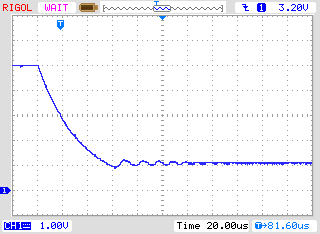
\includegraphics[width=.95\textwidth]{../PNG/AREF2_1V.png}
    \caption{с \(5~V\) до \(1,1~V\)}
    \label{pic:aref1}
  \end{subfigure}
  ~
  \begin{subfigure}[b]{.5\textwidth}
    \centering
    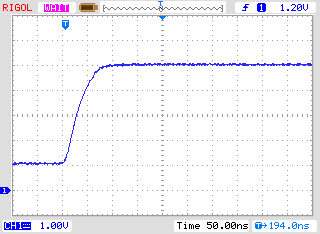
\includegraphics[width=.95\textwidth]{../PNG/AREF2VCC.png}
    \caption{с \(1,1~V\) до \(5~V\)}
    \label{pic:aref5}
  \end{subfigure}
  \caption{Переключение AREF с ёмкостью \(1~nF\)}
\end{figure}
  \item[REF\_R\_KORR] gibt einen Offset für die interne Referenz-Spannung in mV-Einheiten an.
Mit diesem Offset kann eine Differenz bei der Umschaltung der Referenzspannung\\
f?r die Widerstandsmessung abgeglichen werden.
Wenn die AUTO\_CAL-Option gewählt wurde, ist dieser Wert nur ein Offset zu der gefundenen Spannungs-Differenz in der
AUTO\_CAL Funktion.\\
Beispiel: CFLAGS += -DREF\_R\_KORR=10

  \item[OP\_MHZ] Сообщает программному обеспечению, на какой частоте в \(MHz\) будет функционировать Ваш Тестер. 
Программное обеспечение проверено только на \(1~MHz\), \(8~MHz\) и, дополнительно, на \(16~MHz\). \(8~MHz\) 
рекомендуется для лучшего разрешения при измерении ёмкости и индуктивности.\\
Пример: OP\_MHZ = 8

  \item[RESTART\_DELAY\_TICS] Если ATmega168 или ATmega328 используются с внутренним RC-генератором вместо кварца, 
то величина установки должна быть 6. Если это значение не установлено, то при выходе из SLEEP MODE ATmega с 
кварцем, программное обеспечение отсчитывает задержку в 16384 такта.\\
Пример: CFLAGS += -DRESTART\_DELAY\_TICS=6

  \item[USE\_EEPROM] Опция позволяет использовать для размещения фиксированного текста и таблиц память EEprom. 
В противном случае используется программная память Flash. Рекомендуется использовать память 
EEprom (опция установлена).\\
Пример: CFLAGS += -DUSE\_EEPROM

  \item[EBC\_STYLE] Опция задает стиль отображения результатов при определении назначения выводов элементов. 
Если активна опция CFLAGS += -DEBC\_STYLE то информация о расположении выводов транзистора будет 
отображаться относительно назначения выводов, например: \inquotes{EBC=231} или \inquotes{EBC =312}. Опция вида 
CFLAGS += -DEBC\_STYLE=321 позволяет закрепить вывод информации относительно обратного расположения 
тестовых портов в приборе, например: \inquotes{321=BCE} или \inquotes{321=EBC}. Если эти опции не активны, то формат вывода 
будет базироваться относительно тестовых выводов в порядке \inquotes{123=...}, например: \inquotes{123=BCE} или
\inquotes{123=EBC}.\\
Пример: CFLAGS += -DEBC\_STYLE
 
  \item[NO\_NANO] Определяет, что десятичная приставка \inquotes{nano} не будет использоваться при отображении измеренных 
результатов. Значения отображаются в \(\mu F\) вместо \(nF\).\\
Пример: CFLAGS += NO\_NANO

  \item[NO\_LONG\_PINLAYOUT] позволяет избежать длинного стиля отображения назначения выводов \inquotes{~Pin~~1=E~2=B~3=C}.
  Если опция установлена, используется короткий стиль отображения назначения выводов \inquotes{~Pin~~123=EBC}.\\
Пример: CFLAGS += NO\_LONG\_PINLAYOUT

  \item[PULLUP\_DISABLE] Определяет, что Вы не нуждаетесь во внутренних подтягивающих резисторах. Если Вы выбрали 
эту опцию, то у Вас должен быть установлен внешний резистор с вывода PD7 (вывод~13) к VCC. Эта опция предотвращает 
возможное влияние подтягивающих резисторов на результаты измерений в измерительных портах (порт~B и порт~C).\\
Пример: CFLAGS += -DPULLUP\_DISABLE

  \item[ANZ\_MESS] Эта опция определяет количество считанных значений АЦП для вычисления среднего значения. 
Вы можете выбрать любое значение между 5 и 200 для подсчета среднего значения одного измерения АЦП. Более 
высокие значения дают большую точность, но увеличивают время измерения. Одно среднее значение измерений АЦП 
со значением 44 требует приблизительно \(5~ms\).\\
Пример: CFLAGS += -DANZ\_MESS=55

  \item[POWER\_OFF] Эта опция включает функцию автоматического выключения питания. Если Вы не установите эту опцию, 
измерения будут идти бесконечно, пока не будет отключено питание прибора. Если у Вас Тестер без 
схемы отключения питания, то Вы можете не выбирать POWER\_OFF.
Если Вы не установили опцию POWER\_OFF для прибора с авто отключением, то Тестер можно выключить из меню 
выбора функций при активизированной опции WITH\_MENU.
Вы можете также определить, после скольких измерений без определения элемента Тестер выключится. Тестер также 
отключит питание после вдвое большего числа измерений, сделанных последовательно без неудавшегося поиска элемента. 
Это позволяет избежать полного разряда батареи, если Вы забыли отсоединять тестируемый элемент. Выбор определяется 
как CFLAGS += -DPOWER\_OFF=5 для 5 последовательных измерений без определения элемента. Тестер также выключится 
после 10 измерений с определением элемента. Если любая последовательность измерений будет прервана другим типом, 
то измерения продолжатся. Результат измерения отображается на дисплее в течение 28 секунд для однократного 
измерения, для многократного измерения время отображения уменьшено до 5 секунд (выбор в config.h). Если кнопка 
\textbf{ TEST} нажата более длительное время, то время отображения для многократного измерения также 28~секунд. 
Максимальное значение 255 (CFLAGS += -DPOWER\_OFF=255).\\
Пример 1: CFLAGS += -DPOWER\_OFF=5\\
Пример 2: CFLAGS += -DPOWER\_OFF

  \item[BAT\_CHECK] Позволяет проверять напряжение батареи питания. Если Вы не выбираете эту опцию, то на  
LCD-дисплее вместо напряжения будет отображаться номер версии программного обеспечения. Эта опция полезна для 
версии Тестера, работающей от автономного источника питания, чтобы напомнить о разряде источника питания.\\
Пример: CFLAGS += -DBAT\_CHECK

  \item[BAT\_OUT] Позволяет отображать напряжение батареи на LCD-дисплее (если выбрана опция BAT\_CHECK). Если 
в цепи питания \(9~V\) установлен диод, то для правильного измерения выходного значения необходимо учесть напряжение 
падения на нем (в \(mV\)), для этого используйте  BAT\_OUT =600. Также этой опцией можно учитывать падение напряжения 
на транзисторе T3. Пороговый уровень не влияет на уровни проверки напряжения (BAT\_POOR).\\
Пример 1: CFLAGS += -DBAT\_OUT=300\\
Пример 2: CFLAGS += -DBAT\_OUT

  \item[BAT\_POOR] Установка нижнего уровня напряжения батареи, задаваемого в \(mV\). 
Если нижний уровень составляет больше чем \(5,3~V\), то уровень предупреждения о разряде батареи на \(0,8~V\) выше, 
чем указанный нижний уровень. 
Если нижний уровень составляет \(5,3 V\) или менее, то уровень предупреждения о разряде батареи на \(0,4~V\) выше, 
чем указанный нижний уровень. 
Если нижний уровень ниже \(3,25~V\), то уровень предупреждения о разряде батареи на \(0,2~V\) выше, чем указанный 
нижний уровень. 
Если нижний уровень ниже \(1,3~V\), то уровень предупреждения о разряде батареи на \(0,1~V\) выше, чем указанный 
нижний уровень. 
Установка нижнего уровня \(5,4~V\) не рекомендуется для перезаряжаемых \(9~V\) аккумуляторов, потому что это 
увеличивает риск повреждения аккумулятора из-за глубокого разряда! Если Вы хотите использовать \(9~V\) аккумулятор, 
то рекомендуется использовать Ready To Use тип аккумулятора из-за более низкого саморазряда.\\
Пример для low drop regulator (\(5,4~V\)): CFLAGS += -DBAT\_POOR=5400\\
Пример для 7805 type regulator (\(6,4~V\)): CFLAGS += -DBAT\_POOR=6400

  \item[DC\_PWR] Уровень напряжения в \(mV\) измеренного при тесте напряжения питания Тестера, выше
  которого устанавливается режим \inquotes{DC\_Pwr\_Mode}. Обычно Тестер работает от батареи и при этом все 
дополнительные функции ограничены во времени. В режиме \inquotes{DC\_Pwr\_Mode}, предполагается, что Тестер работает 
от внешнего блока питания, поэтому дополнительные функции работают без ограничения по времени.
Потому что DC-DC преобразователь не работает при входном напряжении меньше \(0.9~V\),
режим \inquotes{DC\_Pwr\_Mode} также устанавливается, если обнаружено напряжение питания батареи ниже \(0.9~V\). \\
Пример: CFLAGS += -DDC\_PWR=9500

  \item[BAT\_NUMERATOR] значение числителя сокращённой дроби при расчёте резистивного делителя для измерения напряжения 
батареи. В рекомендованном делителе напряжения, состоящего из резистора \(10~k\Omega\) и резистора \(3.3~k\Omega\), 
Вы получите следующее выражение: \(\frac{ 10000 + 3300}{ 3300} = \frac{ 133}{ 33}\). \\
Пример: CFLAGS += -DBAT\_NUMERATOR=133

  \item[BAT\_DENOMINATOR] значение знаменателя из сокращённой дроби при расчёте резистивного делителя 
для измерения напряжения батареи. \\
Пример: CFLAGS += -DBAT\_DENOMINATOR=33

  \item[EXT\_NUMERATOR] значение числителя сокращённой дроби при расчёте резистивного делителя для измерения внешнего 
входящего напряжения.
Если делитель состоит из резистора \(180~k\Omega\) и резистора \(20~k\Omega\), то соотношение будет:
\(\frac{ 180000 + 20000}{ 20000}\).
После сокращения дроби получим: \(\frac{ 10}{ 1}\). \\
Пример: CFLAGS += -DEXT\_NUMERATOR=10

  \item[EXT\_DENOMINATOR] значение знаменателя сокращённой дроби при расчёте резистивного делителя для измерения 
внешнего входящего напряжения. \\
Пример: CFLAGS += -DEXT\_DENOMINATOR=1

  \item[INHIBIT\_SLEEP\_MODE] Запрещает использование SLEEP\_MODE. Обычно программное обеспечение 
использует SLEEP\_MODE для более длительной работы. Использование этого способа действительно экономит 
заряд батареи, но создает дополнительную нагрузку для стабилизатора напряжения.\\
Пример: INHIBIT\_SLEEP\_MODE = 1 (для версий до 290)\\
Пример: INHIBIT\_SLEEP\_MODE = 0 (для версии 291 и выше)
\label{sec:config-Prog}
  \item[PROGRAMMER] \label{PROGRAMMER}устанавливает тип программатора для интерфейсной программы \lcmd{avrdude}.\\

Необходима правильная установка типа программатора (и порта). \\
В Makefile по умолчанию установлен программатор из Diamex. \\
USBasp от Fischler и Arduino Mega также готовятся. \\
Если должен использоваться другой программист, он должен быть включен в Makefile и, до настоящего момента, отменен с помощью \# ~ в начале строки. \\
Пример использования USBtiny Programmer: \\
\# настройка для USBtiny ISP\\
PROGRAMMER=usbtiny\\
BitClock=10\\
PORT=usb\\
и еще один пример:\\
\#~настройка для программиста Pololu\\
\#~PROGRAMMER=stk500v2\\
\#~BitClock=1.0\\
\#~Port = /dev/ttyACM0\\
Пример: PROGRAMMER=avrisp2


  \item[BitClock] Выбирает частоту синхронизации для программатора. См. описание -B параметра для \lcmd{avrdude}.\\
Пример: BitClock=5.0

  \item[PORT] Выбранный порт, через который Ваш микроконтроллер ATmega может быть доступным для \lcmd{avrdude}. За 
дополнительной информацией обратитесь, пожалуйста, к описанию avrdude.\\
Пример: PORT=usb

\end{description}

Дополнительные параметры могут быть установлены в файлах \lname{transistortester.h} и \lname{config.h}.
Файл \lname{config.h} содержит глобальные переменные и определяет порт/контакт и величину резистора,
которые используются для измерения. Файл \lname{transistortester.h} определяет параметры для различных типов микроконтроллеров, задержку и частоту АЦП. Обычно нет 
необходимости изменять эти значения.

% Microcontroller Programming
\section{Программирование микроконтроллера}
Я публикую программное обеспечение для микроконтроллера ATmega с исходным кодом.
Разработка сделана в среде операционной системы Linux (Ubuntu) и компилируется с помощью \lname{Makefile}.
\lname{Makefile} даёт уверенность, что программное обеспечение будет корректно скомпилировано
у Вас с предварительно выбранными опциями в \lname{Makefile}.
Некоторые структуры предкомпилированы с исходником.
Пожалуйста, смотрите  \lname{ReadMe.txt} файл в каталоге \lname{Software/default} 
и главу~\ref{sec:config} на странице~\pageref{sec:config}.
Результат компиляции представлен файлами с двумя расширениями \lname{.hex} и \lname{.eep.}
По умолчанию имена будут \lname{TransistorTester.hex} и \lname{TransistorTester.eep}.
Файл с расширением \lname{.hex} содержит данные для памяти программ (Flash), 
а файл с расширением \lname{.eep} содержит данные для памяти EEprom  микроконтроллера ATmega.
Оба файла с данными должны быть загружены в соответствующие области памяти микроконтроллера ATmega.\\

Дополнительные опции состояния микроконтроллера ATmega должны быть запрограммированы фьюзами.
Если Вы можете использовать мой Makefile с программой \lcmd{avrdude} \cite{avrdude},
Вам не нужны детальные знания о фьюзах. 
Вы должны только выбрать \lcmd{make fuses} , если у Вас нет кварца,s
или \lcmd{make fuses-crystal} , если Вы установили кварц на \(8~MHz\) на свою печатную плату.

С серией ATmega168 Вы можете также использовать, \lcmd{make fuses-crystal-lp} , 
чтобы использовать кварц с низким потреблением мощности.
Никогда не выбирайте установки с кварцем, если кварц на \(8~MHz\) либо \(16~MHz\) у Вас не установлен.

Если Вы не уверены с фьюзами, оставляете их заводскими и приведите Тестер в рабочее 
состояние в этом режиме.
Работа программы может замедлиться, если Вы используете программные данные,
определенные для работы на \(8~MHz\), но Вы сможете исправить это позже!
А вот неправильный выбор фьюзов может запретить в будущем ISP-программирование.
Конечно, программа \lcmd{avrdude} должна поддерживать ваш программатор, и конфигурация в \lname{Makefile} 
должна соответствовать Вашей среде разработки.\\

% use under Linux
\subsection{использовать под Linux}
К отчаянию и \inquotes{бессонным ночам}, которые Шрайбер перенес из этой главы, после чего он, не имея опыта AVR, приобрел тестер клонов и хотел \inquotes{научить} немецкому языку, чтобы пощадить других коллег. написал эту главу.
Приобретенный здесь опыт должен помочь другим \inquotes{желающим} неопытным людям
 
УСПЕШНО программировать тестера. \\
Эта возможность используется разработчиком тестера транзисторов и автором этого документа,

Карл-Хайнц Кюббелер благодарит \cite {karlheinz1} за его преданность и терпение \\
потому что следующие страницы никогда не были бы созданы без его помощи.
     
Так что прошивка может быть скомпилирована и записана в MCU и одновременно \dots \\
\inquotes{Колесо не нужно было бы заново изобретать}, было частью следующих страниц
Оригинал взят.

Итак, еще раз \dots \ огромный {СПАСИБО ОГРОМНОМУ}
\ нормализует Карла-Хайнца Кюббелера.
% Operating System Linux
\subsection{операционная система Linux}
Программирование под Linux имеет много преимуществ, потому что эта ОС была разработана экспертами, которые ориентированы на пожелания пользователей.
Кроме того, среда доступна бесплатно и отлично поддерживается.

Еще одним преимуществом является безопасность как самой ОС, так и при использовании Интернета. \\
Сегодняшние издания намного проще в использовании, чем их конкуренты, ОС. \\
Это руководство предназначено для того, чтобы побудить всех \inquotes{не} пользователей Linux протестировать его СЕЙЧАС, запрограммировав свой тестер.

В качестве примера используется текущая версия Linux Mint из Интернета.
\\ Установка возможна по-разному и поставляется с собственным менеджером загрузки, чтобы вы могли продолжать использовать существующую ОС параллельно.
% use under Linux
\subsection{использовать под Linux}
как новая ОС. \\
Для тех, кто не любит писать, есть простой способ.

Скопируйте это руководство на USB-накопитель и откройте его в Linux. \\
Затем подведите указатель мыши к названию документа, то есть к тексту (\lname{ttester.pdf}),
нажмите левую кнопку мыши и перетащите документ к левому краю экрана, пока не отобразится возможный кадр.
Теперь мышь отпущена.

Теперь инструкции занимают левую половину экрана.
% install software packages 
\subsection{установить программные пакеты}
Для программирования тестера сначала должны быть установлены программные пакеты: \\
'binutils-avr', 'avrdude', 'avr-libc' и 'gcc-avr'.

Теперь перейдите на эту страницу до этого текста:

\begin{large} \vspace{-0.4em} \begin{verbatim}
sudo apt-get install avrdude avr-libc binutils-avr gcc-avr git
\end{verbatim} \end{large}
На следующем шаге одновременно нажимаются \keys{{Ctrl} + \Alt + T}, чтобы открыть командное окно.
Теперь это перемещено к правому краю экрана таким же образом.

Пометьте вышеупомянутый текст в левом окне, удерживая левую кнопку мыши
\\ поместите мышь на курсор правого командного окна и нажмите

с помощью средней кнопки мыши (колесо прокрутки) \textbf {снова сокращенно обозначаем как [MT]}.\\
После подтверждения нажатием \keys{Enter} \lcmd{sudo} по-прежнему будет запрашивать пароль пользователя.

Теперь все программные пакеты установлены \inquotes{apt}. \\
U.U. между ними вы должны подтвердить вопросы с помощью [J].
\\ Пожалуйста, убедитесь, что Linux различает прописные и строчные буквы.
\\ Так что не отвечайте с [jo], но с [J]!
% download of sources
\subsubsection{Скачать исходный код}
Было ли успешно установлено управление версиями \ lcmd {git},
можно проверить с помощью следующей команды: 
\begin{large} \vspace{-0.4em} \begin{verbatim}
git version
\end{verbatim} \end{large}
Программа \lcmd{git} должна ответить выводом номера своей версии.
Если папка transistortester уже существует в вашем домашнем каталоге,
вам следует переименовать или удалить ее.
Программа \lcmd{git} используется для загрузки исходников и документации.
С помощью команды:

\begin{large} \vspace{-0.4em} \begin{verbatim}
git clone https: //github.com/Mikrocontroller-net/transistortester
\end{verbatim} \end{large}
скачивается полный архив. \\
Теперь файлы следуют в [личной папке] Linux, обычно это \lname{/home/}.
от вашего идентификатора пользователя с именем каталога \lname{transistortester}.
С помощью терминального ввода \lcmd{ls} \(\mbox{\keys{L} \keys{S} \keys{\return}} \) вы можете
проверить наличие.
Вы можете получить больше информации о файлах и каталогах с помощью
команда \lcmd{ls -lh}. 
Здесь объединены две опции для команды \lcmd{ls}: опция \lcmd{{-l}} и опция \lcmd{{-h}}.
Таким образом, эта форма ввода является краткой формой для
команда \lcmd{ls -l -h} или \lcmd{ls -l --human-readable}.
Некоторые параметры представлены в двух версиях: короткой форме с одной - (\lcmd{{-h}}) и длинной
форме с двумя - (\lcmd{{ --human-readable}}).
Кстати, порядок опций значения не имеет,
точно так же, как количество разделительных пробелов \keys{\space}.
Почти для всех команд вы можете узнать больше об операции и параметрах, добавив параметр \lcmd{{--help}}.
Конечно, это также относится к команде \lcmd{git}. \\
Чтобы загрузить новые обновления, в будущем будет достаточно ввестиs
\begin{large} \vspace{-0.4em} \begin{verbatim}
git pull
\end{verbatim} \end{large}
в рабочий каталог \lname{transistortester}. 
В зависимости от интерпретатора команд это также можно сделать с помощью
\begin{large} \vspace{-0.4em} \begin{verbatim}
(cd ~/transistortester ; git pull)
\end{verbatim} \end{large}
из каждого рабочего каталога.
Чтобы \lcmd{git pull} работал правильно, лучше не менять дерево каталогов.

% Compiling of transistortester sources
\subsubsection{Перевести исходники тестера транзисторов}

Для компиляции исходных кодов тестера транзисторов требуется только вызов \lcmd{make}
в правильном рабочем каталоге.
Поскольку ATmega также может быть запрограммирована с подключенным
программатором ISP с помощью \lcmd{make upload},
имеет смысл сначала разобраться с интерфейсами для подключения программатора ISP.
Дальнейший рабочий процесс описывается в пункте~\ref{sec:Arbeitsumgebung} на
странице~\pageref{sec:Arbeitsumgebung}. 


% use of interfaces
\subsubsection{использование интерфейсов}
подготовить для пользователя.
Устройства USB можно распознать, введя \lcmd{lsusb} в командном окне.
Сначала введите \lcmd{lsusb}, а затем подключенный USB-программатор. \\
Сравнение результатов локализует USB-программатор.

Результат \lcmd{lsusb} может выглядеть так:
\begin{footnotesize} \begin{verbatim}
Bus 001 Device 001: ID 1d6b:0002 Linux Foundation 2.0 root hub
Bus 002 Device 003: ID 046d:c050 Logitech, Inc. RX 250 Optical Mouse
Bus 002 Device 058: ID 03eb:2104 Atmel Corp. AVR ISP mkII
Bus 002 Device 059: ID 2341:0042 Arduino SA Mega 2560 R3 (CDC ACM)
Bus 002 Device 001: ID 1d6b:0001 Linux Foundation 1.1 root hub
\end{verbatim} \end{footnotesize}
Здесь AVR ISP mkII был распознан как Устройство 58 (DIAMEX ALL-AVR). \\
ID 03eb - это идентификатор производителя, а ID 2104 - это идентификатор продукта. \\
Эти два идентификатора необходимы для файла \lname{/etc/udev/rules.d/90-atmel.rules} и созданы \\
с помощью:

\begin{large} \vspace{-0.4em} \begin{verbatim}
sudo xed /etc/udev/rules.d/90-atmel.rules
\end{verbatim} \end{large}
В этом примере файл \lname{90-atmel.rules} состоит из одной строки:
\begin{verbatim}
SUBSYSTEM=="usb", ATTRS{idVendor}=="03eb", ATTRS{idProduct}=="2104", MODE="0660",
GROUP="plugdev"
\end{verbatim}
Эта запись разрешает доступ к устройству для членов группы \lname{plugdev}. \\
~ \\
Чтобы использовать большинство программистов, рекомендуется следующий текст на 90-atmel.rules:
\begin{verbatim}
# Copy this file to /etc/udev/rules.d/90-atmel.rules
# AVR ISP mkII - DIAMEX ALL-AVR
SUBSYSTEM=="usb", ATTRS {idVendor}=="03eb", ATTS {idProduct}=="2104", MODE="0660", 
 GROUP = "plugdev",
# USB ISP-programmer f?r Atmel AVR
SUBSYSTEM=="usb", ENV {DEVTYPE}=="usb_device", SYSFS {idVendor}=="16c0", MODE="0666",
 SYSFS {idProduct} == "05dc",
# USB asp programmer
ATTRS {idVendor}=="16c0", ATTRS {idProduct}=="05dc", GROUP="plugdev", MODE="0660"
# USBtiny programmer
ATTRS {idVendor}=="1781", ATTRS {idProduct}=="0c9f", GROUP="plugdev", MODE="0660"
# Pololu programmer
SUBSYSTEM=="usb", ATTRS {idVendor}=="1ffb", MODE="0666"
\end{verbatim}
После того, как файл был создан, вы можете проверить создание и содержание с:

меньше \lname{/etc/udev/rules.d/90-atmel.rules} \\
Системное USB-устройство Arduino SA Mega 2560, также распознаваемое как Устройство 59, генерирует одно
Доступ к последовательному устройству \lname{/dev/ttyACM0} для членов группы \lname{dialout}.
% group membership
\subsection{членство в группе}
Следовательно, ваш собственный идентификатор пользователя также должен быть членом группы \lname{plugdev}
группа \inquotes{дозвон}. Команда:

\begin{large} \vspace{-0.4em} \begin{verbatim}
sudo usermod -a -G dialout,plugdev $USER
\end{verbatim} \end{large}
должен обеспечить принадлежность.
Avrdude теперь должен иметь доступ к обоим устройствам.
Вы можете проверить это с помощью команды: \lcmd{id}. \\
В случае возникновения проблем, членство также может быть сделано через: \\
~ Меню /Системное администрирование/Пользователи и группы/<Пароль>/появится окно с двумя вкладками. \\
Если вы теперь щелкните по его имени на вкладке \inquotes{Пользователь}, вы увидите его профиль и принадлежность к группе справа.
С помощью кнопки <ADD> теперь можно добавлять новые группы.

\subsection{Рабочая среда и перевод источников}
\label{sec:Arbeitsumgebung}
Чтоб сохранился оригинал, рекомендуется создавать дубликаты источников с именем \textbf{Mytester}.
Обычно домашний каталог называется \lname{/home/}, за которым следует ваш идентификатор пользователя.
Имя вашего домашнего каталога хранится в системной переменной \lname{\$HOME}.
Вы также можете для краткости писать \lname{\textasciitilde/} вместо имени в командах.
Не забывайте \lname {/} после символа \lname{\textasciitilde},
иначе интерпретатор команд будет искать пользователя со следующим именем!
Для этого сначала создайте пустой каталог с:
\begin{large} \vspace{-0.4em} \begin{verbatim}
mkdir ~/Mytester
\end{verbatim} \end{large}
Если вы скачали из архива в каталог \lname{\textasciitilde/transistortester},
вы можете выполнить следующую команду, чтобы скопировать исходные файлы и их подкаталоги в каталог Mytester. 
\begin{large} \vspace{-0.4em} \begin{verbatim}
rsync -auv ~/transistortester/Software/trunk/ ./Mytester
\end{verbatim} \end{large}
Из-за параметра \lcmd{-v} \lcmd{rsync} регистрирует все процессы копирования.
Если вы укажете \lcmd{-au} в качестве параметров вместо параметров \lcmd{-auv}, процесс копирования останется безмолвным.
Убедиться в заполнении подкаталога trunk можно с помощью следующей команды:
\begin{large} \vspace{-0.4em} \begin{verbatim}
ls -lh ~/Mytester/trunk
\end{verbatim} \end{large}
Четкое отображение структуры каталогов и файлов возможно с помощью команды \lcmd{tree \textasciitilde/Mytester}.
Команда не устанавливается по умолчанию, что легко сделать с помощью \lcmd{sudo apt-get install tree}. \\

Если теперь вы знаете, какой подкаталог подходит для вашего тестера,
вы можете перейти в этот подкаталог.
Предположим, у вас есть китайский комплект с программным дисплеем,
тогда подкаталог \lname{mega328\_st7565\_kit} будет правильным.
Тогда команда для этого будет:
\begin{large} \vspace{-0.4em} \begin{verbatim}
cd ~/Mytester/trunk/mega328_st7565_kit
\end{verbatim} \end{large}
Вы также можете просмотреть файлы в \lname{\textasciitilde/Mytester/trunk/} с помощью окна
файлов \menu[,]{menu, accessories, files},
каталог \lname{Mytester}, а затем \lname{trunk} можно выбрать двойным щелчком \LMB. 
Теперь здесь появляется много подкаталогов, в том числе
желаемое \lname{mega328\_st7565\_kit}.
Если вы теперь также выберете этот каталог двойным щелчком по \LMB,
вы также можете увидеть \lname{Makefile} под файлами
Если вы это сделали, теперь вы можете использовать клавишу \RMB для выбора
функции \menu{Открыть в терминале}, и откроется командное окно с правильным рабочим каталогом,
который также непосредственно активен.
Теперь вам нужно только ввести \lcmd{make}, и он программа тестера транзисторов перевела снова.
Теперь у вас есть два окна, которые уже находятся в правильном рабочем каталоге.
Окно файлов и окно терминала для ввода команды \lcmd{make}.
Если \ LNB дважды щелкнуть файл \lname{Makefile} в окне файлов, откроется другое окно с редактором предустановок.
Если вы предпочитаете другой редактор, вы можете
выберите этот редактор либо напрямую через \RMB \menu[,]{{Открыть с помощью}}.
Если вы всегда хотите установить другой редактор для текстовых файлов,
это также можно сделать через \RMB \menu[,]{Properties}.
Затем открывается новое окно \verb"Свойства файла Makefile",
в котором вы можете выбрать функцию \menu[,]{{Открыть с помощью}}, щелкнув \RMB.
Здесь вы можете увидеть текущую настройку и выбор параметров для редактирования \lname{Makefile}.
Здесь вы можете выбрать другое приложение, нажав \LMB.
Щелкнув \LMB, вы можете теперь выбрать, хотите ли вы использовать это
приложение: \menu[,]{{Добавить в список}} или \menu[,]{{Использовать по умолчанию}}.
Вы также можете снова использовать \menu[,]{{Восстановить системные значения по умолчанию}}.
Для следующего шага важно, чтобы настройки для
\textbf{ваш ISP-программист}, в котором \lname{Makefile} установлен правильно.
См. Также в подразделе \ref{sec:config} на странице \pageref{sec:config-Prog},
Тема \textbf{PROGRAMMER} и \textbf{PORT}.
Когда вы проверите эти настройки,
вы можете повторно активировать окно терминала, щелкнув \LMB.
Когда окно активировано, заголовок имеет более высокий контраст!
Если ваш ISP-программатор теперь полностью подключен, то есть имеет соединение с компьютером и ATmega,s
вам нужно только ввести команду:
\begin{large} \vspace{-0.4em} \begin{verbatim}
make upload
\end{verbatim} \end{large}
Теперь программа тестера транзисторов компилируется снова и сразу же загружается в ATmega с помощью
программы \lcmd{avrdude}.
Вам не нужно каждый раз вводить команду.
Команды, уже введенные в окне терминала, можно снова отобразить с помощью клавиши \keys{arrowkeyup}.
Вы можете повторить отображаемую команду, нажав клавишу \keys{\enter} или \keys{\return}.
Но вы также можете отредактировать отображаемую команду перед ее отправкой,
или переключитесь на новые команды с помощью \keys{arrowkeydown}.\\


Наконец, здесь снова перечислены наиболее важные вызовы \lname{Makefile}: 
\begin{table}[H]
%  \begin{center}
   \begin{tabular}{ l | l}
   Инструкция               & смысл \\
      \hline
\lcmd{make clean}               & очистить рабочую среду \\
\lcmd{make}                     & для компиляции программы \\
\lcmd{make fuses}               & для установки ATmega ,,предохранители'' без кварца \\
\lcmd{make fuses-crystal}       & для установки ATmega ,,fuses'' ТОЛЬКО с версией с \(8MHz\) кварцем!\\
\lcmd{make upload}              & загрузить переведенную программу через интерфейс ISP в ATmega\\
   \end{tabular}
%  \end{center}
%  \caption{}
%  \label{}
\end{table}

\subsubsection{Примечания по обновлению исходников тестера транзисторов}
Копию источников транзисторного тестера можно обновлять с помощью команды:
\begin{large} \vspace{-0.4em} \begin{verbatim}
(cd ~/transistortester ; git pull)
\end{verbatim} \end{large}
Если вы работаете с копией под \lname{\textasciitilde/Mytester}, как рекомендовано здесь,
изменения будут перенесены только в том случае, если вы также выполните команду:
\begin{large} \vspace{-0.4em} \begin{verbatim}
rsync -auv ~/transistortester/Software/trunk ~/Mytester
\end{verbatim} \end{large}
Может случиться так, что \lname{Makefile} на сервере github имеет более новую дату, чем локально измененная копия.
Тогда изменения, внесенные в параметры в \lname{Makefile} локально в папке Mytester, будут потеряны.
Поэтому рекомендуется сохранить успешно измененный файл \lname{Makefile} как копию.
Это можно сделать, например, с помощью команды \lcmd{cp Makefile Makefile.bak}.
Затем вы можете использовать команду \lcmd{diff Makefile Makefile.bak}
позвольте компьютеру сравнить файлы после обновления.
Более подробный обзор изменений также возможен с помощью \lcmd{kdiff3 Makefile Makefile.bak}.
Программа должна быть установлена с помощью \lcmd{sudo apt-get install kdiff3},
потому что на самом деле она была разработана для среды рабочего стола KDE.

\newpage

\subsection{Использование программы WinAVR в ОС Windows}
Если Вы используете операционную систему Windows, то самый легкий способ получить правильно запрограммированный ATmega 
состоит в том, чтобы использовать пакет WinAVR \cite{winavr1},\cite{winavr2}.
Для установки фьюзов с помощью Makefile Вы можете использовать мой Patch for WinAVR  \cite{winavr3}\\

На рисунке~\ref{fig:WinAVR1} показано меню File графического интерфейса пользователя WinAVR для открытия файла 
Makefile (Open) и для того, чтобы сохранить изменённый Makefile (Save).

\begin{figure}[H]
  \begin{subfigure}[b]{.5\textwidth}
    \centering
    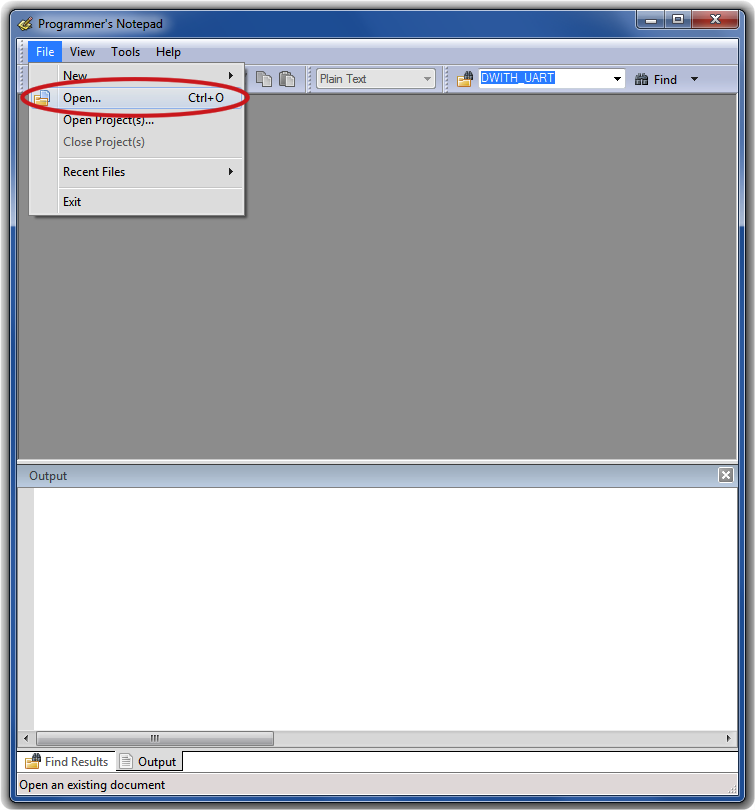
\includegraphics[width=.95\textwidth]{../PNG/Notepad_open.png}
    \caption{Открыть Makefile}
  \end{subfigure}
  ~
  \begin{subfigure}[b]{.5\textwidth}
    \centering
    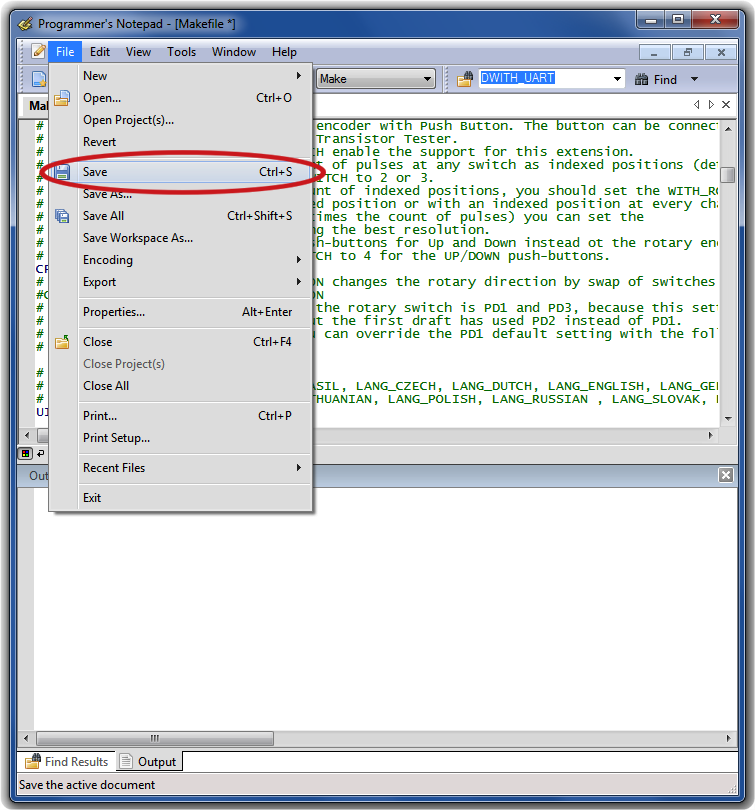
\includegraphics[width=.95\textwidth]{../PNG/Notepad_save.png}
    \caption{Сохранить Makefile}
  \end{subfigure}
  \caption{Использование программы WinAVR}
  \label{fig:WinAVR1}
\end{figure}

Следующий рисунок~\ref{fig:WinAVR2} показывает меню Tools графического интерфейса пользователя WinAVR для того, чтобы 
скомпилировать программу (Make All) и для того, чтобы запрограммировать ATmega (Program) программой avrdude.

\begin{figure}[H]
  \begin{subfigure}[b]{.5\textwidth}
    \centering
    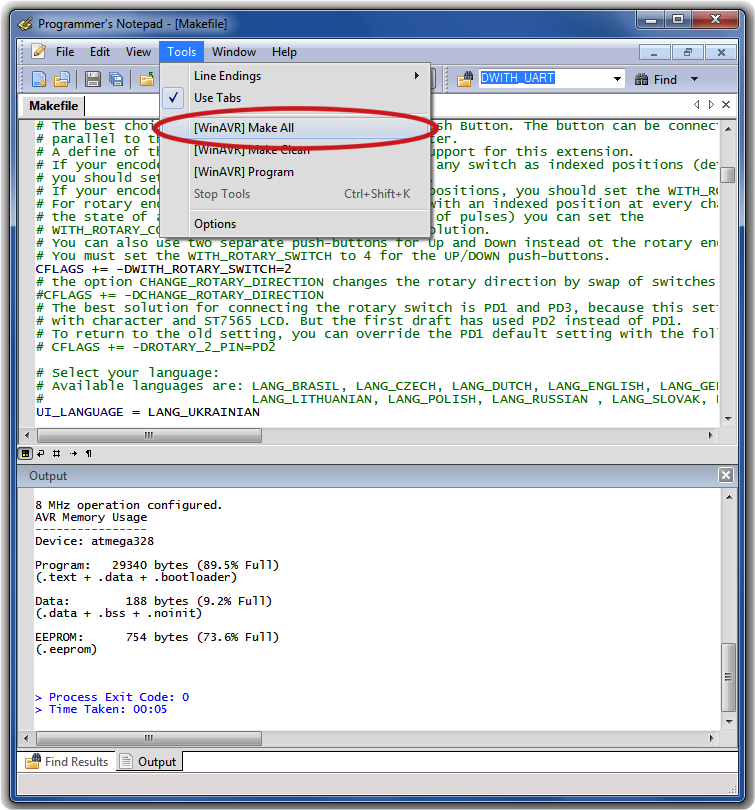
\includegraphics[width=.95\textwidth]{../PNG/Notepad_make.png}
    \caption{Создание прошивки (.hex/.eep)}
  \end{subfigure}
  ~
  \begin{subfigure}[b]{.5\textwidth}
    \centering
    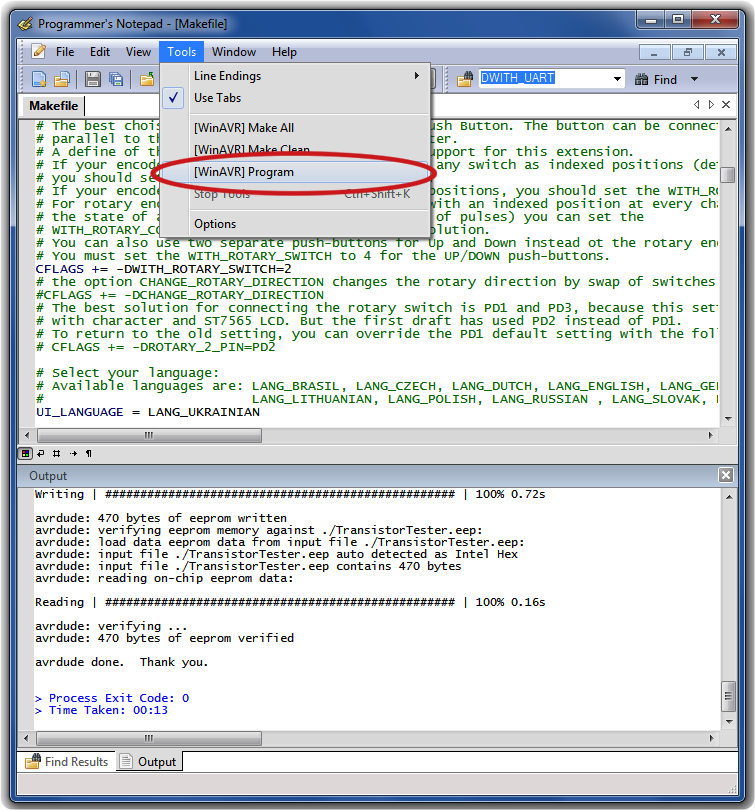
\includegraphics[width=.95\textwidth]{../PNG/Notepad_program.png}
    \caption{Программирование ATmega}
  \end{subfigure}
  \caption{Использование WinAVR}
  \label{fig:WinAVR2}
\end{figure}

\section{Поиск неисправностей }
В большинстве случаев возникают проблемы с выводом текста на LCD-дисплей. Сначала Вы должны проверить, что светодиод 
LED1 не светится, если Вы отпускаете кнопку \textbf{ TEST}. 
\begin{description}

\item[Питание не включается.]
Если светодиод LED1 не светится, и VCC = \(5~V\) во время нажатия кнопки \textbf{ TEST}, микроконтроллер не включает 
питание. 
В первую очередь, микроконтроллер должен держать питание, переключая уровень PD6 на \(5~V\). Если Вы удерживаете кнопку 
\textbf{ TEST}, питание должно быть включено.
Так Вы можете проверить величину напряжения питания VCC и одновременно величину 
напряжения на PD6. Если напряжения VCC = \(5~V\), а напряжение на PD6 ниже \(4~V\), то микроконтроллер не запускает программу. 
В этом случае Вы должны проверить, был ли микроконтроллер запрограммирован надлежащими данными для установленного у 
Вас типа ATmega во Flash и EEprom, и правильно ли сформированы фьюзы. Если микроконтроллер переводит состояние PD6 в 
\(5~V\), но питание не остается после отпускания кнопки \textbf{ TEST}, то это усложняет поиск причины. Сначала Вы можете замкнуть 
светодиод LED1 и попробовать еще раз. Если Тестер запускается, то светодиод LED1 может быть дефектным или установлен 
с неправильной полярностью. Если причина не эта, то недостаточен коэффициент усиления транзистора T3 (BC557C).

\item[Отсутствует текст на LCD-дисплее.]
Проверьте напряжение на контакте контрастности в LCD-дисплее. Установите значение, определенное в техническом описании
и оптимизируйте для комфортного просмотра. Для некоторых дисплеев может понадобится отрицательное напряжение для
регулировки контраста. В этом случае Вы можете использовать ICL~7660 для генерации отрицательного напряжения из 
положительного \(5~V\).
Программное обеспечение может быть создано для разных контроллеров и разных интерфейсов подключения
дисплея. Необходимо проверить соответствие установленной программы схеме Вашего тестера и применяемого в нем дисплея.   
Если на LCD-дисплее нет никакой информации, а подсветка есть, то необходимо отключить питание и проверить четыре шины данных 
и две связи управляющих сигналов. Если всё нормально, единственной причиной, которую я вижу, является неправильный 
выбор временных параметров управляющих сигналов. Это может быть вызвано более медленным контроллером LCD-дисплея, чем 
заложено в программном обеспечении или работой программного обеспечения на неправильной тактовой частоте ATmega. 
Необходимо проверить, для какой тактовой частоты были скомпилированы программные данные и соответствуют ли фьюзы 
выбранной частоте ATmega. Вы найдёте параметр частоты в соответствующей строке Makefile. Если Тестер собран без 
отключения, Вы можете проверить работу программы с помощью светодиода, подключенного к испытательным выводам. 
Если светодиод мигает, то программа работает правильно.
Для некоторых графических дисплеев контрастность настраивается из функции в меню. 
Если Вы изменили значение контрастности, так что ничего не читается на экране, Вы можете попробовать увидеть 
информацию на дисплее при просмотре под большим углом, а не спереди. В этом случае Вы можете попробовать 
отрегулировать контрастность из меню. В противном случае, Вы должны переписать данные EEPROM ISP программатором 
для сброса значения контрастности.

\item[Что-то, но не все читаемое на LCD-дисплее.]
Проверить, правильные ли .eep данные загружены в память EEprom  ATmega. Если все данные загружены правильно, 
то необходимо проверить тактовую частоту, программные параметры данных (Makefile) и установки фьюзов ATmega.

\item[Медленное измерение и измеренная ёмкость в 8 раз меньше.] 
Программное обеспечение для \(8~MHz\), а работает ATmega на \(1~MHz\). Проверьте правильность установки фьюзов.

\item[Странные значения измерений.]
Для того, чтобы проводить измерения, ISP программатор должен быть отсоединен. Очень часто причина неправильных 
измерений - использование программного обеспечения, скомпилированного с опцией AUTOSCALE\_ADC и с опцией NO\_REF CAP, 
а на выводе AREF конденсатор ёмкостью \(100~nF\). Неправильный монтаж или остатки флюса также могут нарушить 
измерение. Пожалуйста, если возможно, проверьте функцией самопроверки программное обеспечение Тестера. Подробности 
смотрите в Главе~\ref{sec:selftest}

Осмотрите свою плату визуально и проверьте величины резисторов омметром. Для этой проверки Вы можете использовать 
выводы ATmega, например, чтобы проверить R1, Вы можете провести измерения между выводами 23 и 14 ATmega. Смотрите 
схему на рисунке~\ref{fig:ttester}. Удалять микроконтроллер не обязательно, достаточно только отключить батарею 
или электропитание.

\item[Тестер выключает питание после 2 секунд отображения на дисплее.] 
Это может произойти, если отсутствует внешний подтягивающий резистор с порта PD7 к VCC, или кнопка \textbf{ TEST} 
удерживается нажатой. Программное включение внутренних подтягивающих резисторов влияет на результаты измерения, 
поэтому необходим внешний подтягивающий резистор \(27~k\Omega\). 

\item[Тестер отображает только Vext=xx.xV во второй строке]
Эта проблема появляется, если подтягивающий резистор на выводе PD7
отсутствует, неисправен или кнопка \textbf{ TEST} удерживается в нажатом положении,
а программное обеспечение сконфигурировано с отключением UART (опция WITH\_UART отключена)
и отключенным внутренним подтягивающим резистором (с опцией PULLUP\_DISABLE). 
Необходима установка подтягивающего резистора на выводе PD7.

\end{description}
